\newcommand{\rect}[2]{%
    \fill[lime] (#1-1,0,#2-1) rectangle (#1,0,#2);
}

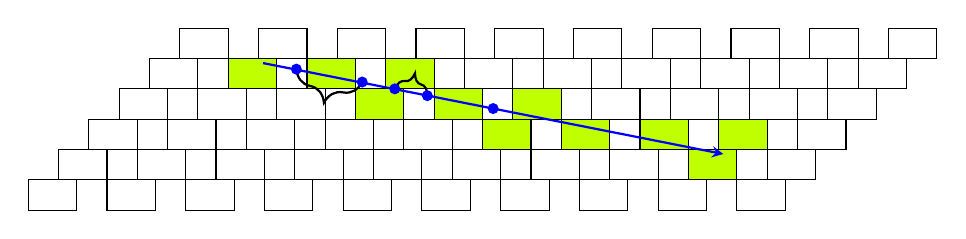
\begin{tikzpicture}[font=\sffamily]
    \rect{2}{2}
    \rect{3}{2}
    \rect{4}{2}
    \rect{4}{3}
    \rect{5}{3}
    \rect{6}{3}
    \rect{6}{4}
    \rect{7}{4}
    \rect{8}{4}
    \rect{9}{4}
    \rect{9}{5}
    % Draw 8×6 grid
    \foreach \x in {0,...,9} {
        \foreach \y in {0,...,5} {
            \draw[black] (\x,0,\y) rectangle (\x+1,0,\y+1);
        }
    }
    \draw[thick, -stealth, blue] (1.5,0,1.15) -- (8.5,0,4.15);

    \coordinate (A) at (2,0,1.35);
    \coordinate (B) at (3,0,1.775);
    \coordinate (C) at (3.5,0,2);
    \coordinate (D) at (4,0,2.225);
    \coordinate (E) at (5,0,2.65);

    \draw[thick, decorate, decoration={brace, amplitude=10pt}] (B) -- (A);
    \draw[thick, decorate, decoration={brace, amplitude=7pt}] (C) -- (D);

    \fill[blue] (A) circle (0.7mm);
    \fill[blue] (B) circle (0.7mm);
    \fill[blue] (C) circle (0.7mm);
    \fill[blue] (D) circle (0.7mm);
    \fill[blue] (E) circle (0.7mm);
\end{tikzpicture}